\clearpage
\newpage
\chapter{Experiments}
In this chapter, we present a comprehensive evaluation of the proposed telehealth system, focusing on its operational efficacy and validation across various experimental setups. The experiments are designed to assess the performance of the collaborative robot in conducting remote physical examinations, emphasising the role of the haptic interface and virtual fixtures in enhancing the teleoperated process. We first detail the experimental setup, highlighting the hardware and software components that facilitate real-time interaction between the physician and patient. Following this, we validate the body model customisation through anthropometric measurements, ensuring accuracy in patient representation. Subsequently, we investigate the effectiveness of the virtual fixtures strategy during lung ultrasound examinations, analysing its impact on both the efficiency and quality of the procedure. Finally, we conduct a thorough validation of the overall lung ultrasound protocol, aiming to quantify the benefits introduced by the telehealth system in a clinical context. Through these experiments, we aim to demonstrate the viability and potential of our telehealth solution in improving remote patient care.


\section{Setup}
\begin{figure}[h]
    \centering
    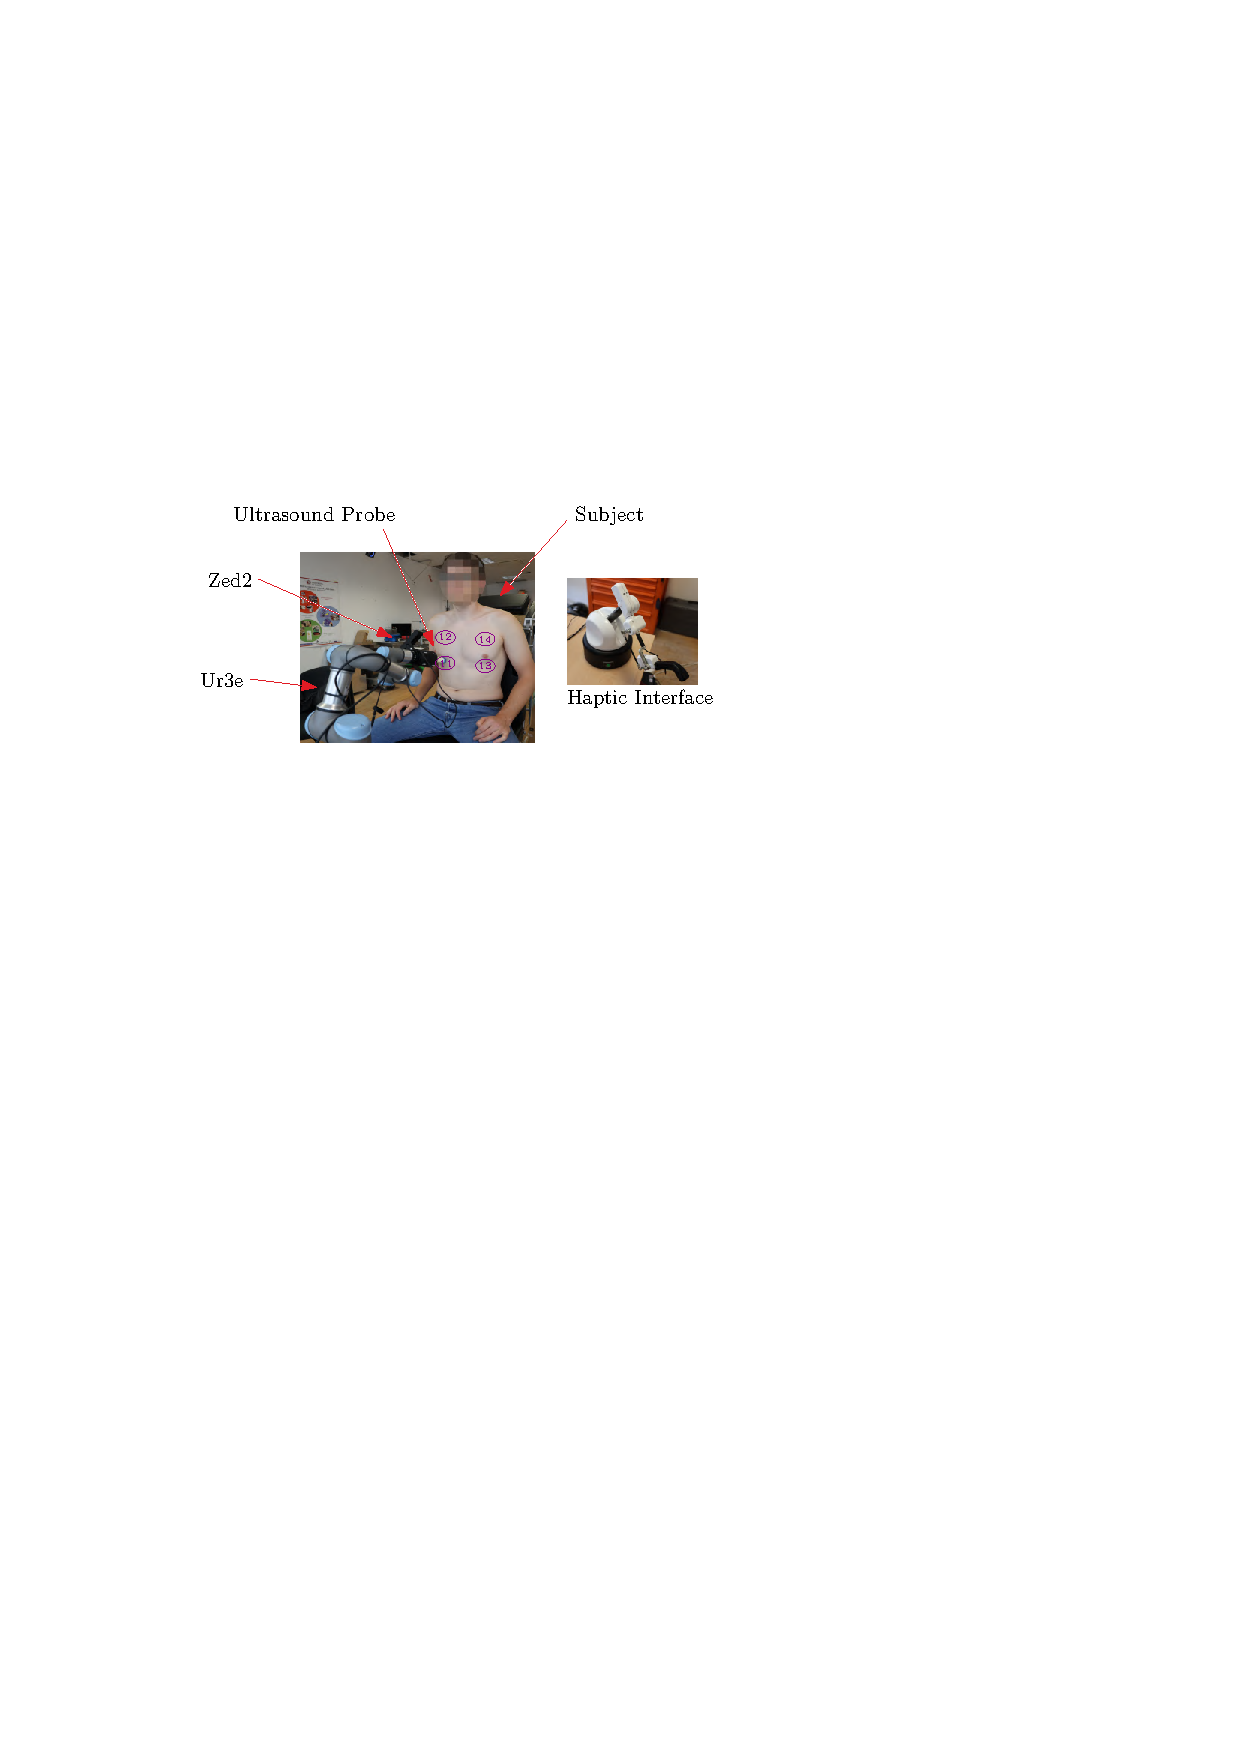
\includegraphics[width=0.9\linewidth]{images/experiments/setup.pdf}
    \caption{Experimental setup: a volunteer male healthy patient sit on an hospital bed and is examinated by a robot arm controlled by the practioner through an haptic interface. The frontal scanning areas of the lung ultrasound protocol considered are marked in purple.   }
    \label{fig:experiments:setup}
\end{figure}

The proposed telehealth system is divided into two main sites. At the patient's side (follower), a collaborative robot endowed with force-torque sensing at the end effector and an ultrasound probe is in charge of the physical examination. 
The robot is teleoperated remotely by a physician by means of a haptic interface (leader), which sends the desired pose to the follower and renders its physical interaction with the environment (the patient's body) through the interface force feedback. Two RGB-D cameras, one mounted at the robot end-effector and the other fixed on a tripod, monitor the robot action and broadcasts its information to the physician's GUIs, which consist, alternatively, of a standard video or a virtual reality interface, that replicates the patient's environment.
The haptic device is a Haption Desktop 6D, which ensures 6 DoFs, plus force and torque feedback and run at 1 khz. The manipulator is a 6-DoFs UR3e controlled at 500 hz with an integrated 6-axis F/T sensor mounted at the robot’s end-effector.  
The robot is controlled using a Forward Dynamics Compliance  controller ~\cite{scherzinger2017forward} which renders an impedance behaviour on kinematically controlled robots. The controller parameters are the following: stiffness $K_{i,i} = 1000, i = 0,...,2$ and $K_{i,i} = 20, i = 3,...,5$, damping $D_{i,i} = 2 \sqrt{K_{i,i}}$, inner PD force controller gains $k_p = 0.05$ and $k_d = 0.005$ for the translation and $k_p = 1.5$ for the rotation, to ensure the force tracking. The RGB-D sensors are a Zed 2 stereo camera mounted on the robot end effector for the 3D model generation and a RealSense 435i fixed on the tripod for the 2D visual feedback.
% To prevent potential patient harm, we will exploit a dummy chest, the Blue Phantom COVID-19 Lung Simulator ($33 cm \times 33 cm \times 23 cm$), which replicates the properties of human tissue, allowing clinicians to practice and develop the ultrasound imaging skills necessary to diagnose the key findings consistent, in this specific case, with COVID-19 cases. The anatomy of the device includes a lung, chest wall, ribs (1–5), and diaphragm. For the palpation exams, we also printed silicon samples with viscoelastic parameters close to those of biological tissues, with internal masses with higher stiffness that represent cancer/foreign masses.
As the end-effector tool we integrated the ATL Wi-Fi US Probe which is attached to the robot flange with a 3D-printed support. We used qpOASES~\cite{ferreau2014qpoases} to solve the mesh-based polygon constraint QP. The radius $r$ of the probe was set to $1$ centimetre. The software components of the framework were communicating through ROS2 Humble installed on Ubuntu 22.04 running on a computer with an AMD Ryzen 9 5900X (24) @ 3.7 GHz × 12-cores CPU, 32 GB RAM, and NVIDIA RTX 4070 GPU.

We facilitated the control of the haptic interface by the integration of a control pad (see \autoref{fig:experiments:control_pad}).
\begin{figure}[h]
    \centering
    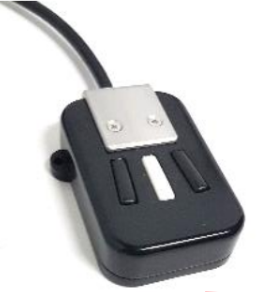
\includegraphics[width=0.35\linewidth]{images/experiments/control_pad.png}
    \caption{The pad used to reposition the haptic interface's handle}
    \label{fig:experiments:control_pad}
\end{figure}
The aluminium plate is a touch sensor that activates the force feedback and pose monitoring when held. Since the workspace is not as large as the real robot arm workspace, it is possible to recentre the handle by releasing the plate.


\section{Validation of the Body Model Customisation}
Since the quality of the skeletal model fitting is strictly related to the SMPL parameters prediction, we evaluated the precision and the accuracy of the algorithm, highlighting the capability of the optimisation of the SMPL model to adapt to different subjects. We considered three anthropometric measurements, related to the body area of interest of this paper:
\begin{enumerate}
    \item chest circumference (CC),
    \item waist circumference (WC),
    \item shoulder to crotch height (SCH).
\end{enumerate}

First, we evaluated the repeatability of the body estimation pipeline
by computing the mean and standard deviation of the anthropometric
measurements in $10$ reconstructions for the same volunteer. The
measurements, obtained with the utility SMPL-Anthropometry~\cite{boja2023smplAnthropometry}, were then compared with the actual measurements taken
from the patient's body with a measuring tape (as in medical
visits). The measures, expressed in metres, are reported in
\autoref{tab:estimation_repeatability}. As we can notice, we obtained
an acceptable standard deviation for our task, especially in the case
of CC, which is also the most relevant among the 3 since it is
measured near the scanning areas: in this case, the standard deviation
is approximately of $3$~cm, which embeds also the low accuracy and
precision of the ground truth measurement method.
%
\begin{table}
    \centering
    \caption{Single subject anthropometric measurements [m] (10 samples)}
    \begin{tabular}{ccc}      \toprule
       \sc{Measurement} & \sc{SMPL (Mean} $\pm$ \sc{std)} & \sc{Measure tape} \\
       \midrule
       CC & 
       0.964 $\pm$ 0.034 & 0.955 \\
       WC &
       0.944 $\pm$ 0.054 & 0.885 \\
       SCH & 0.664 $\pm$ 0.030 & 0.621 \\
       \bottomrule
    \end{tabular}
    \label{tab:estimation_repeatability}
\end{table}
%
% Massa e altezza: 
% - Luca: 1.90 84
% - Davide: 1.75 77
% - Giovanni: 1.81 96.6
% - Edoardo: 1.84 95
%
Then we compared the tape-based measurements with the anthropometric
measurements given by the SMPL model for $4$ male volunteers (only the
male SMPL model is considered), height of
$1.83 \pm 0.05$ metres and mass of $88 \pm 8$
kilograms. The differences between the SMPL and the actual
measurements are shown in
\autoref{tab:estimation_subjectivity}. Notice that, again, we obtained
reasonably low differences, comparable with the ground truth
measurement errors, and with the only exception of CC in patient 2
and WC in patient 4 where outliers can be observed.
\begin{table}[H]
    \centering
    \caption{Anthropometric measurements errors [m] (single sample)}
    \begin{tabular}{cccc}      
       \toprule
       \sc{Subject} & \sc{CC error} & \sc{WC error} & \sc{SCH error}\\
       \midrule
       1 & 0.013 & -0.001 & 0.040 \\
       2 & -0.081 & -0.057 & -0.029 \\
       3 & -0.017 & 0.015 & 0.024 \\
       4 & 0.045 & 0.140 & -0.036 \\
       \bottomrule
    \end{tabular}
\label{tab:estimation_subjectivity}
\vspace{-4mm}
\end{table}
% report mean absolute error
% davide:  [ 1.28869001 -0.1138197   3.99914575]
% edoardo;  [-8.10486383 -5.66265259 -2.94758439]
% luca:  [-1.71130999  1.4861803   2.39914575]


\section{Validation of the Virtual Fixtures Strategy}\label{ssec:exp_fixtures}
To validate the effectiveness of the VF, a lung
ultrasound was performed in the areas of the right basal on
mid-clavicular line below the internipple line (area 11) and of the
right upper on mid-clavicular line above the internipple line (area
12), as proposed by Soldati et al.~\cite{Soldati2020ProposalCOVID-19}
for the standardisation of this examination.
During the examination, the operator, controlling the robot with the
haptic interface, approaches the intercostal space based solely on the
images provided by the RGB camera and the rib reconstruction on the
skinned model. We would like to point out that the presence of the 3D
visual feedback, which includes the fixtures, highly contributes to
assist
%it is anticipated that the visual fixtures will assist 
the physician in reaching the intercostal space, thereby avoiding the
placement of the probe on the bone and the subsequent need for
acquisition correction. In~\autoref{fig:experiments:trajectory_exp2}, and~\autoref{fig:experiments:slicing_exp2}, depicting the outcome of this test, the reference trajectory is generated by the haptic interface, the constrained trajectory is the trajectory with the VF enforcement, and the current trajectory is the position of the robot end effector. The two ultrasound images acquired in the considered areas are shown in \autoref{fig:experiments:scanning-imgs}.

\begin{figure}[h!]
    \centering
    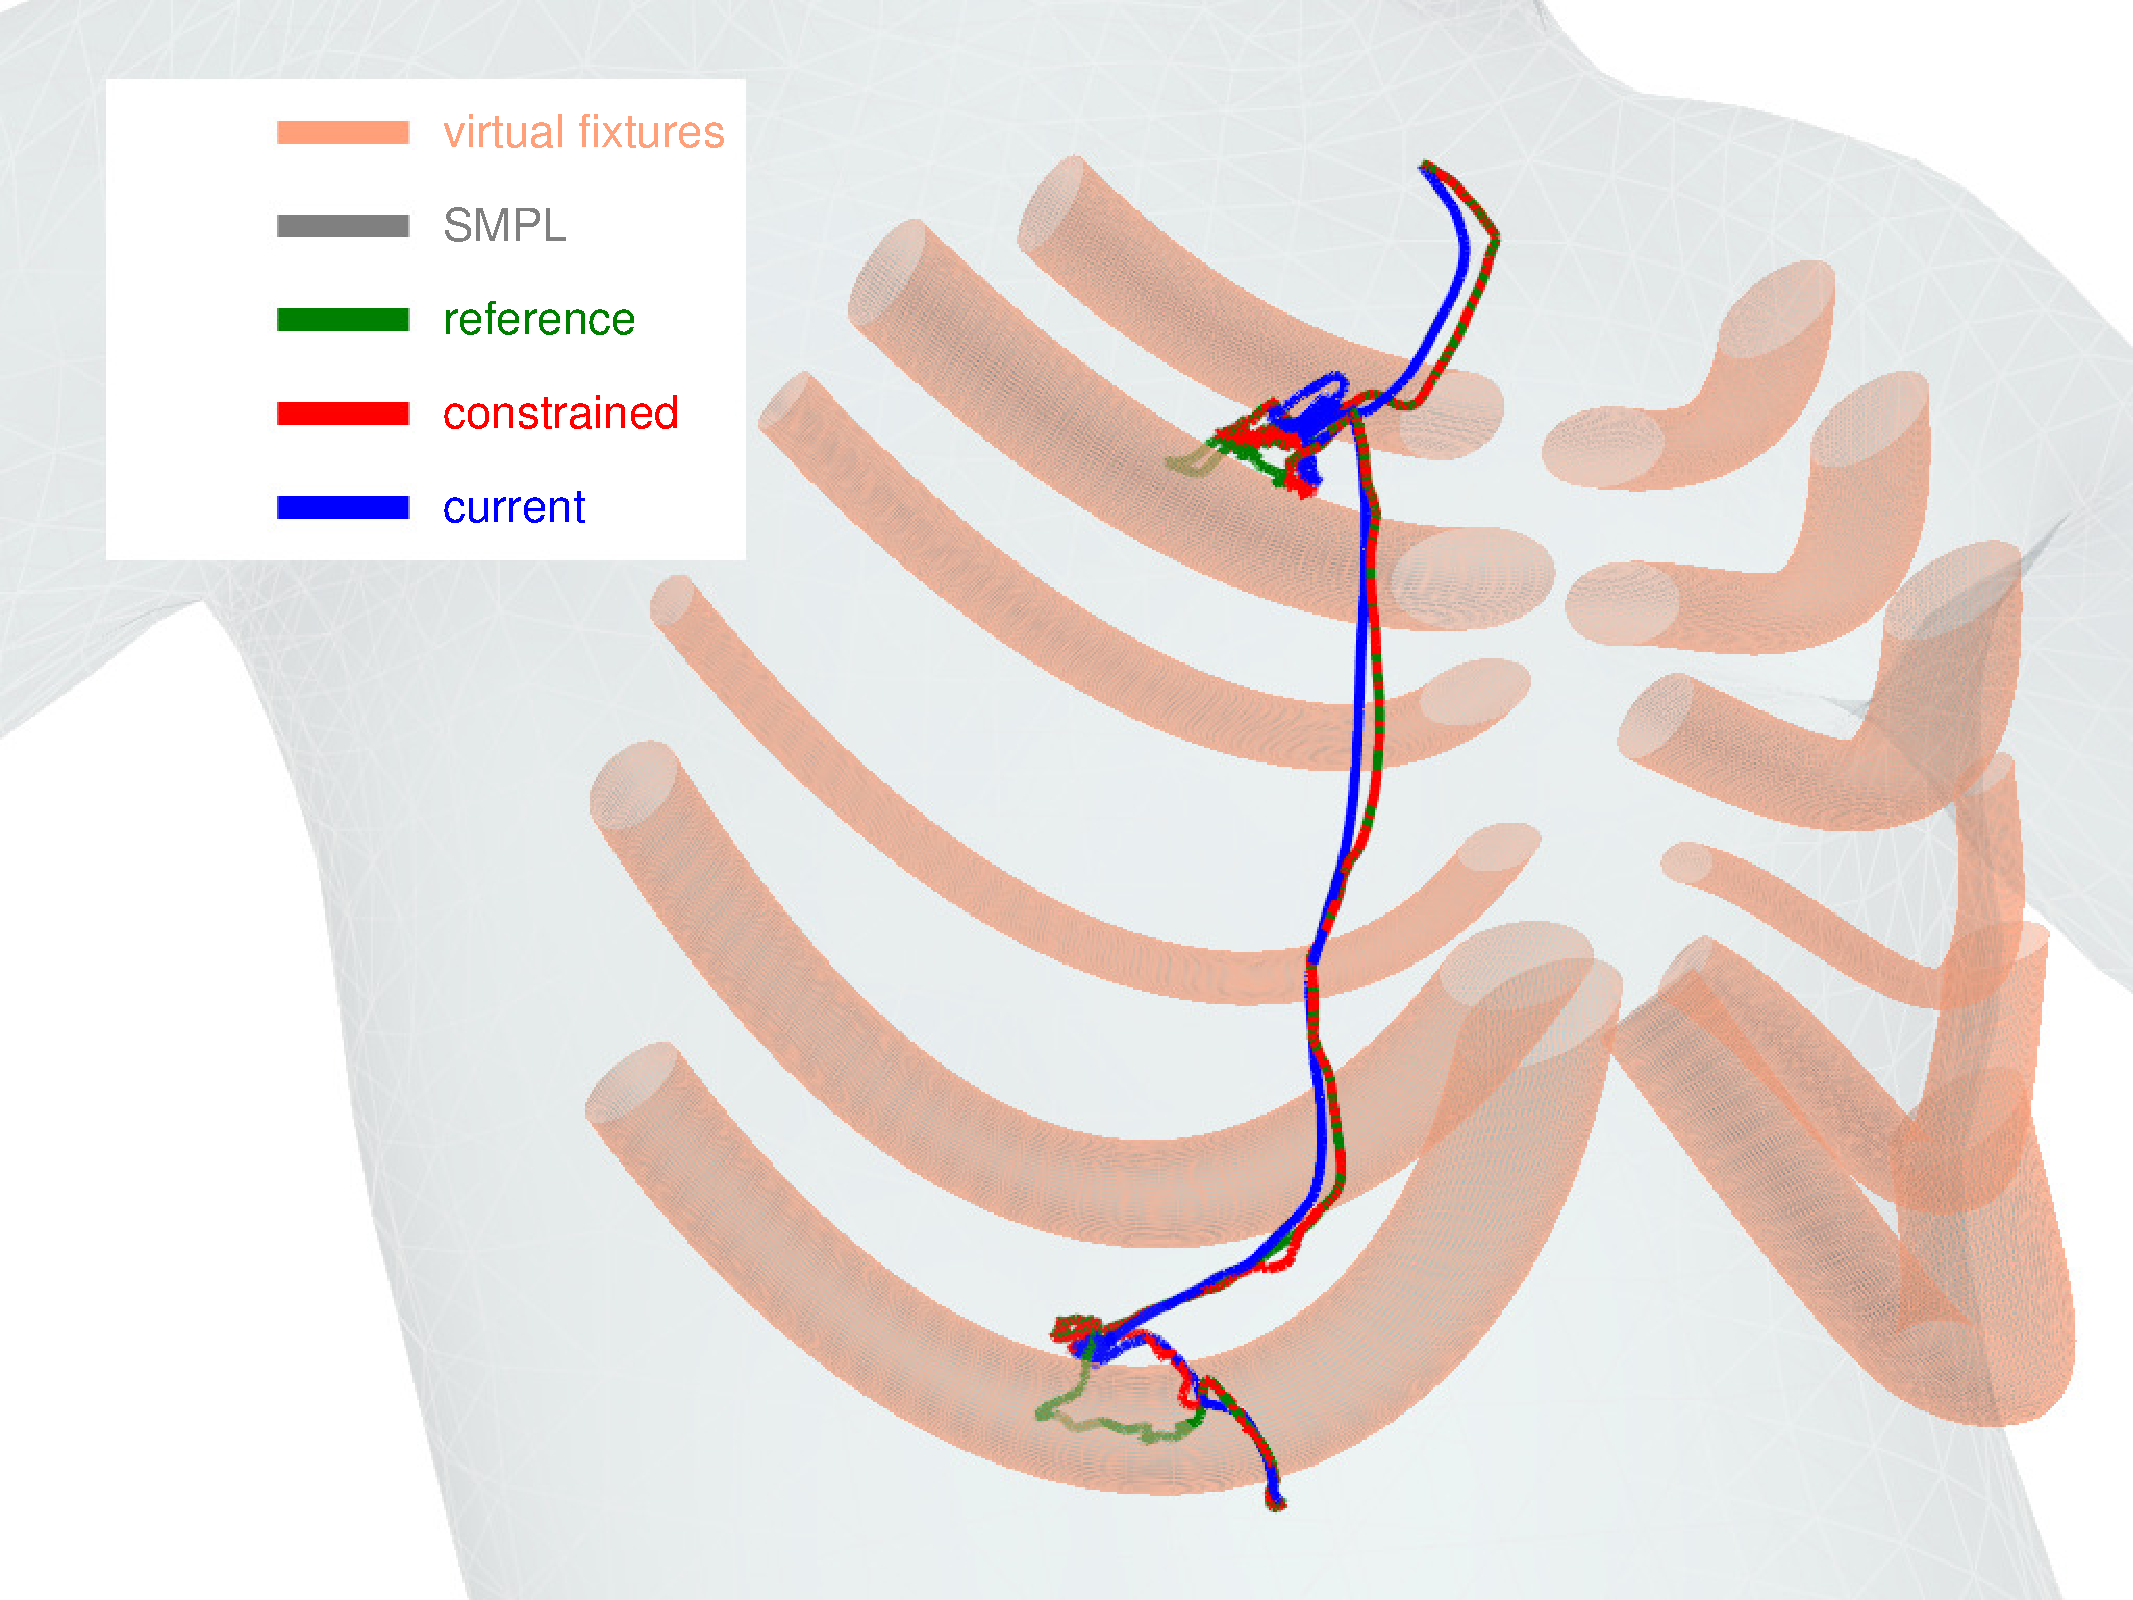
\includegraphics[width=0.6\linewidth]{images/experiments/plot_3D_trajectory_part1.pdf}
    \caption{3D plot of the trajectory measured in experiment 2.}
    \label{fig:experiments:trajectory_exp2}
\end{figure}

\begin{figure}[H]
    \centering
    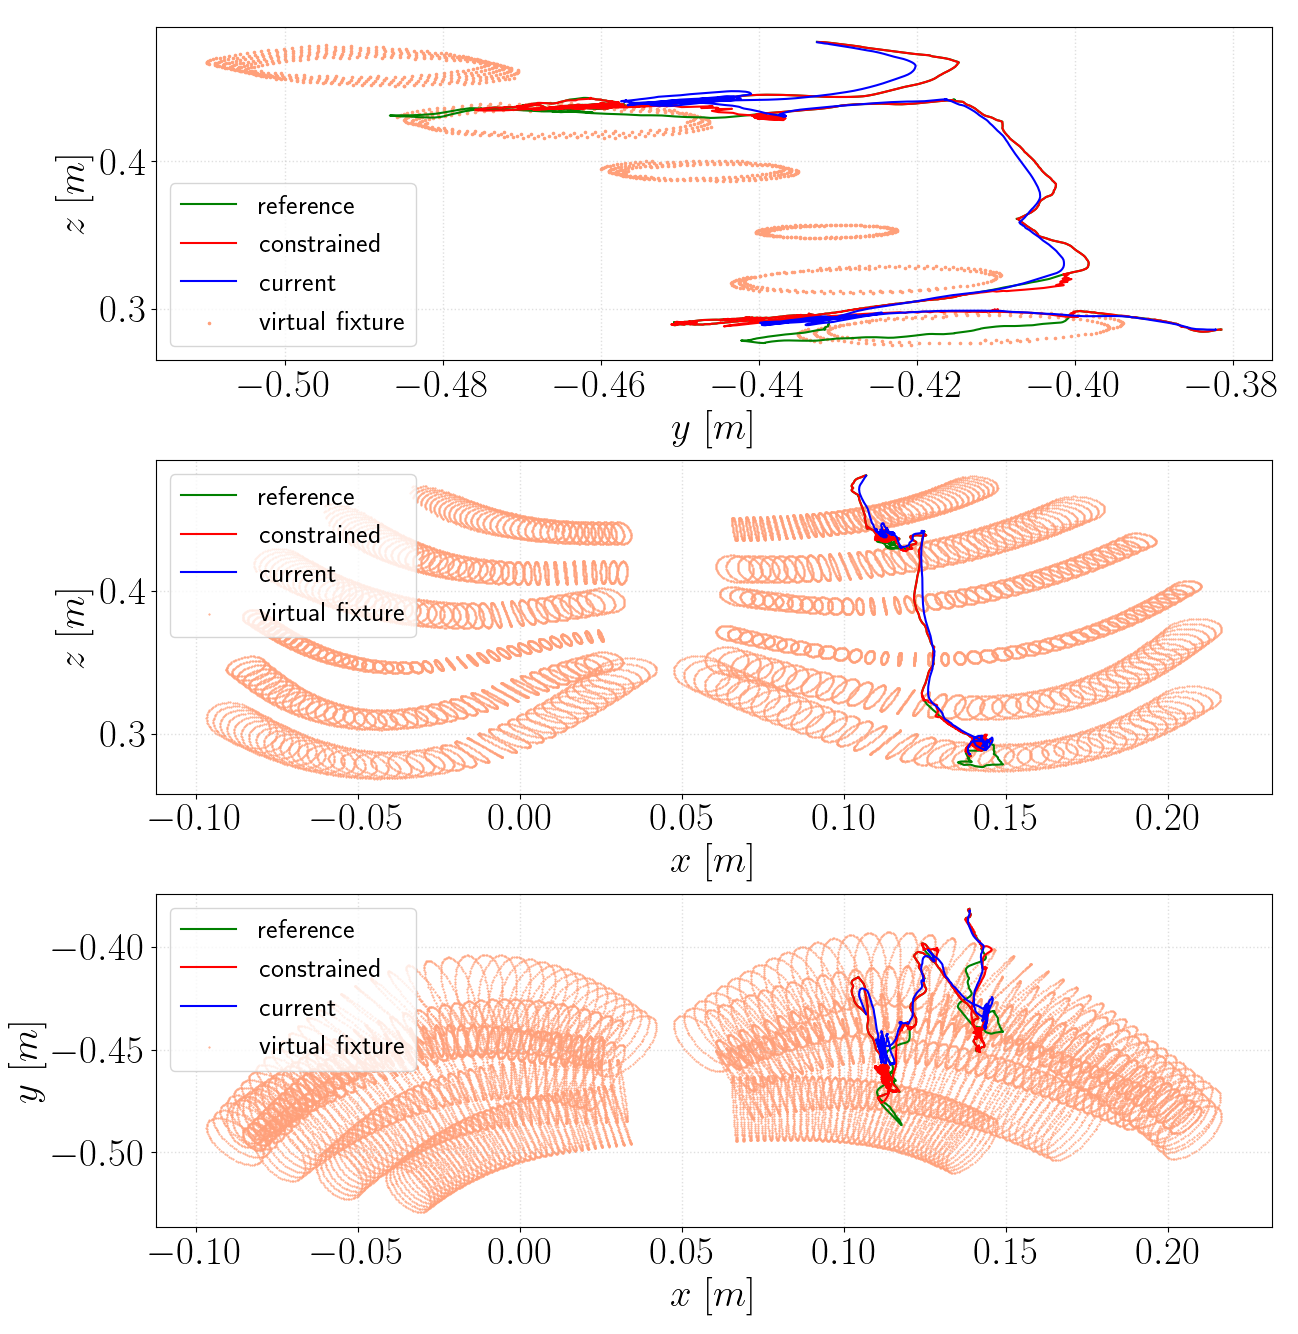
\includegraphics[trim=0cm 0cm 0cm 0cm,clip,width=0.6\linewidth]{images/experiments/plot_slicing.png}
    \caption{2D slices of the 3D plot representing trajectories and VF's ellipses}
    \label{fig:experiments:slicing_exp2}
\end{figure}
\begin{figure}[H]
    \centering
    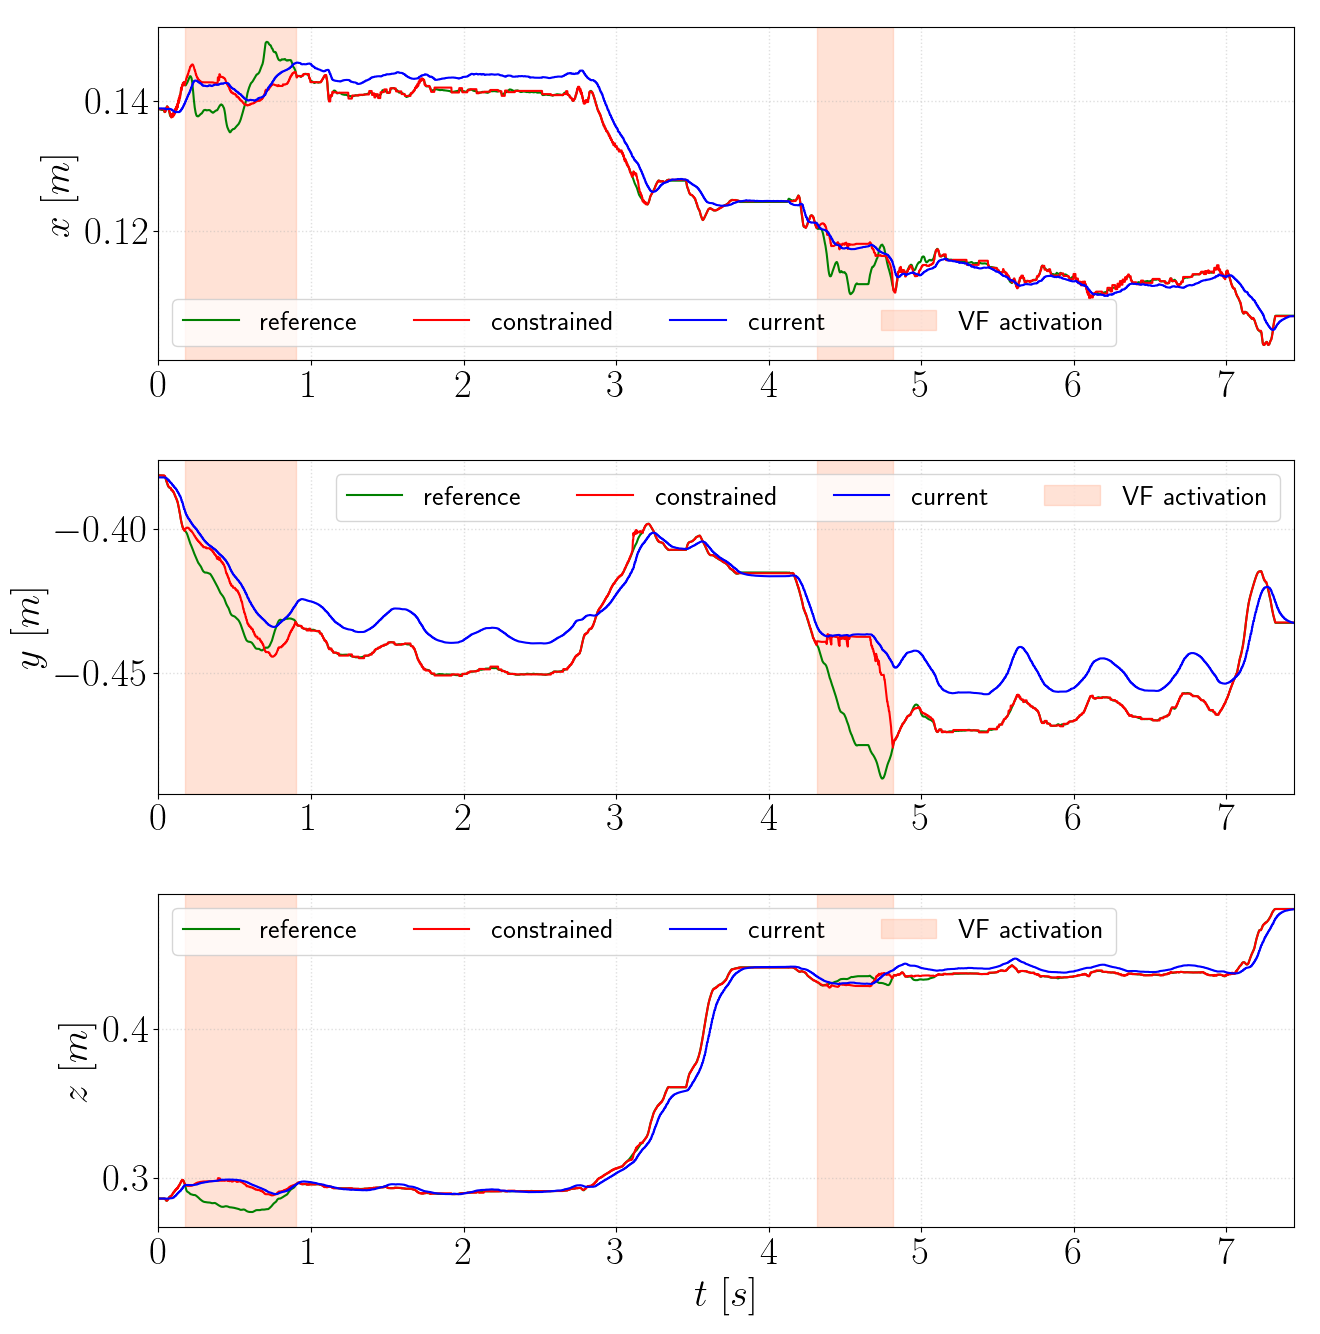
\includegraphics[width=0.6\linewidth]{images/experiments/plot_tracking.png}
    \caption{Trajectories evolution during time for experiment 2, red bars mark the interval in which VF constraint the motion}
    \label{fig:experiments:tracking_exp2}
\end{figure}

% This approach allows for the observation of how the control generates a novel trajectory that circumvents these restricted regions, thereby facilitating a more organic approach phase in which the probe is already in the intercostal zone upon contact with the skin, eliminating the necessity for further user adjustments. 
% The trajectories are displayed in three different formats: on the left, they are shown in a virtual environment; in the centre, they are presented in two dimensions; and on the right, they are displayed in one dimension, with the x-axis representing time. In the latter graph, an examination of the behaviour between 4 and 5 seconds reveals the influence of the virtual fixtures.
With these results, it is possible to observe the activation of the
VF in the presence of a mismatch between the reference
and the constrained trajectory. The green trajectory is the commanded trajectory by the user with the haptic interface, while the constrained is the  one resulting from the enforcement of the virtual fixtures. It is easy to notice that when the reference trajectory pierces the virtual fixtures, the constrained trajectory separate from the reference, indicating a correct VF activation. \autoref{fig:experiments:tracking_exp2} shows the same effect, marked by light red bars.
\begin{figure}
    \centering
    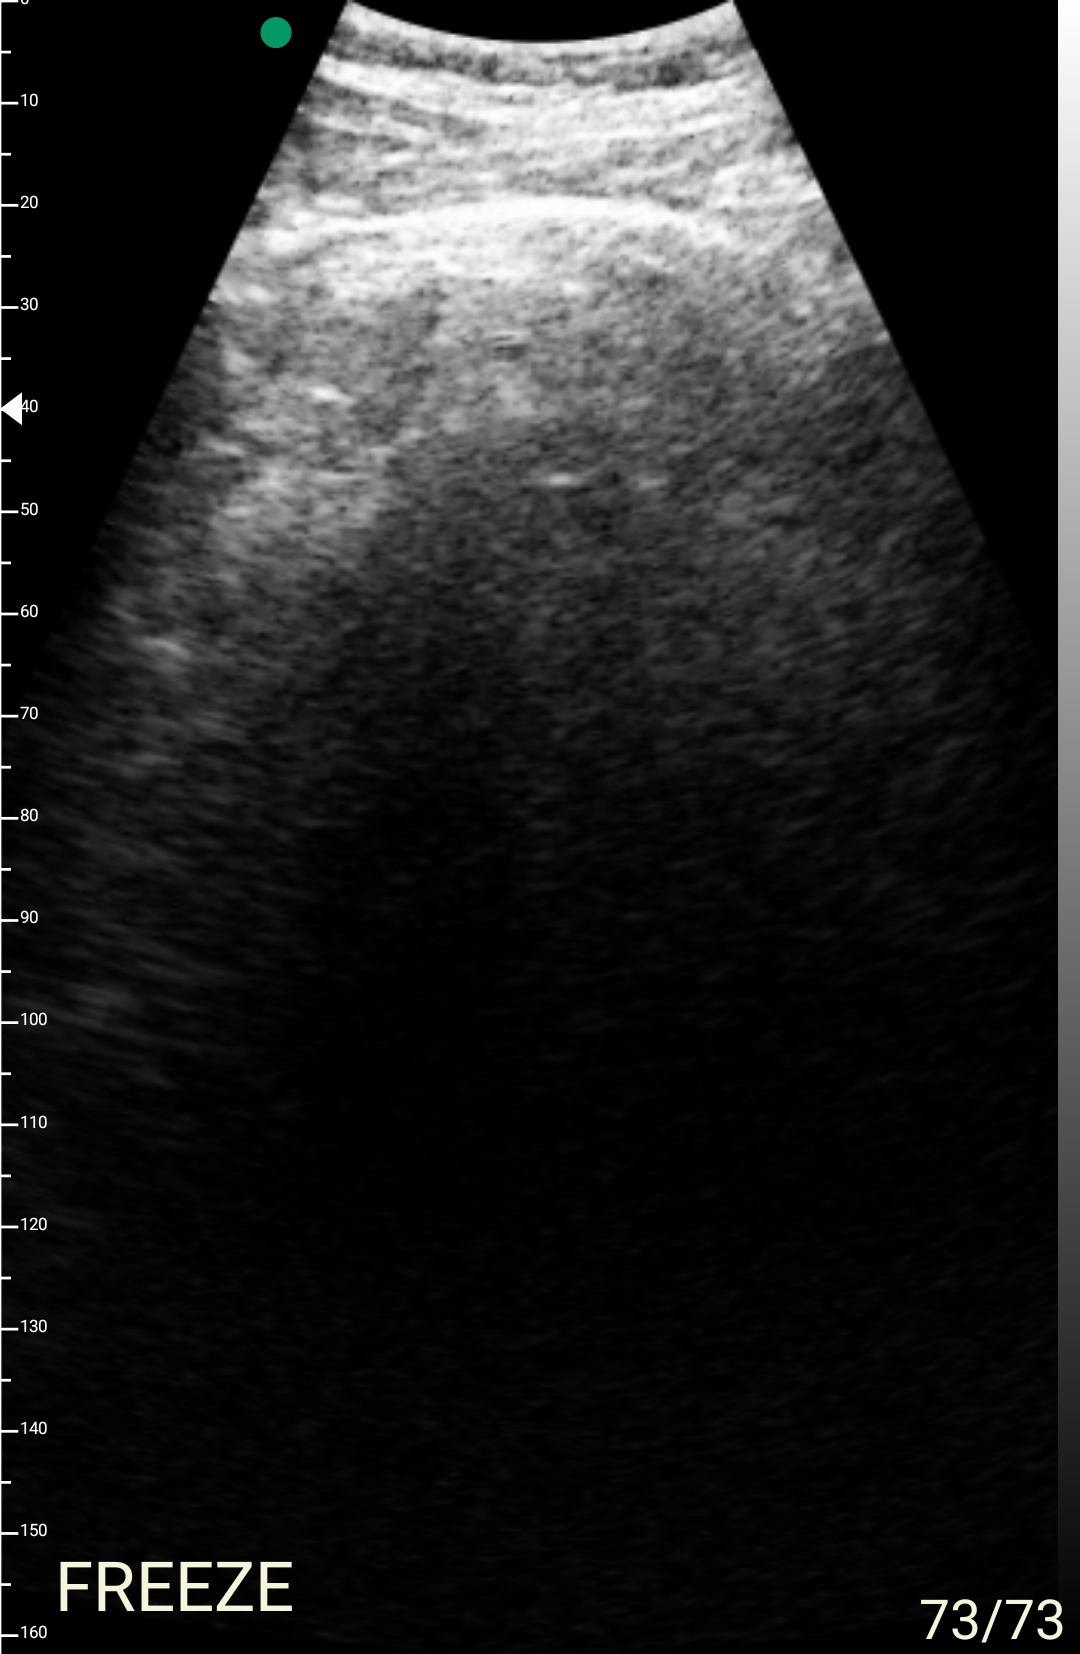
\includegraphics[height=7cm]{images/experiments/11_vf.jpg}
    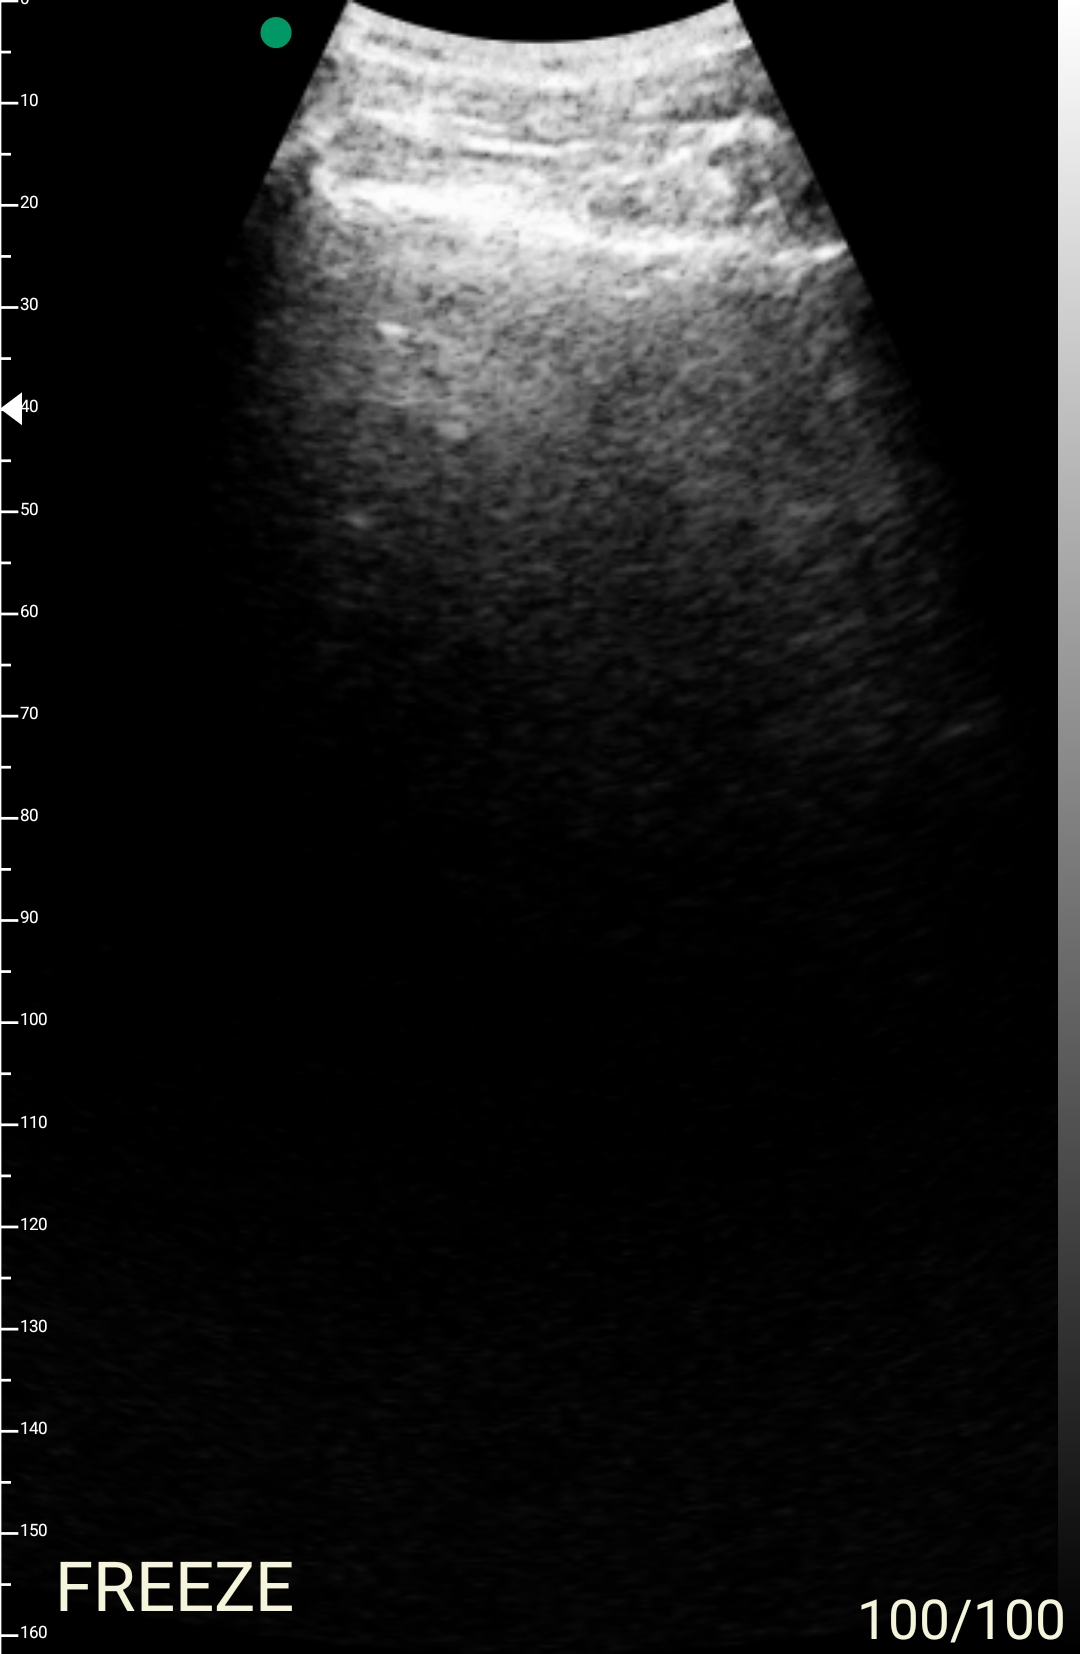
\includegraphics[height=7cm]{images/experiments/12_vf.jpg}
    \caption{Ultrasound image acquired in the areas 11 and 12 of experiment 2. The pleural line is the well-visible thickest white line}
    \label{fig:experiments:scanning-imgs}
\end{figure}
\section{Overall Validation with Lung Ultrasound Protocol}
In light of the challenges associated with the objective assessment of the influence of VF on the acquisition of ultrasound images and the lack of image-based metrics to evaluate the quality of such images, the advantages of the proposed methodology were evaluated based on the duration of the examinations.
% \begin{figure}[h]
%     \centering
%     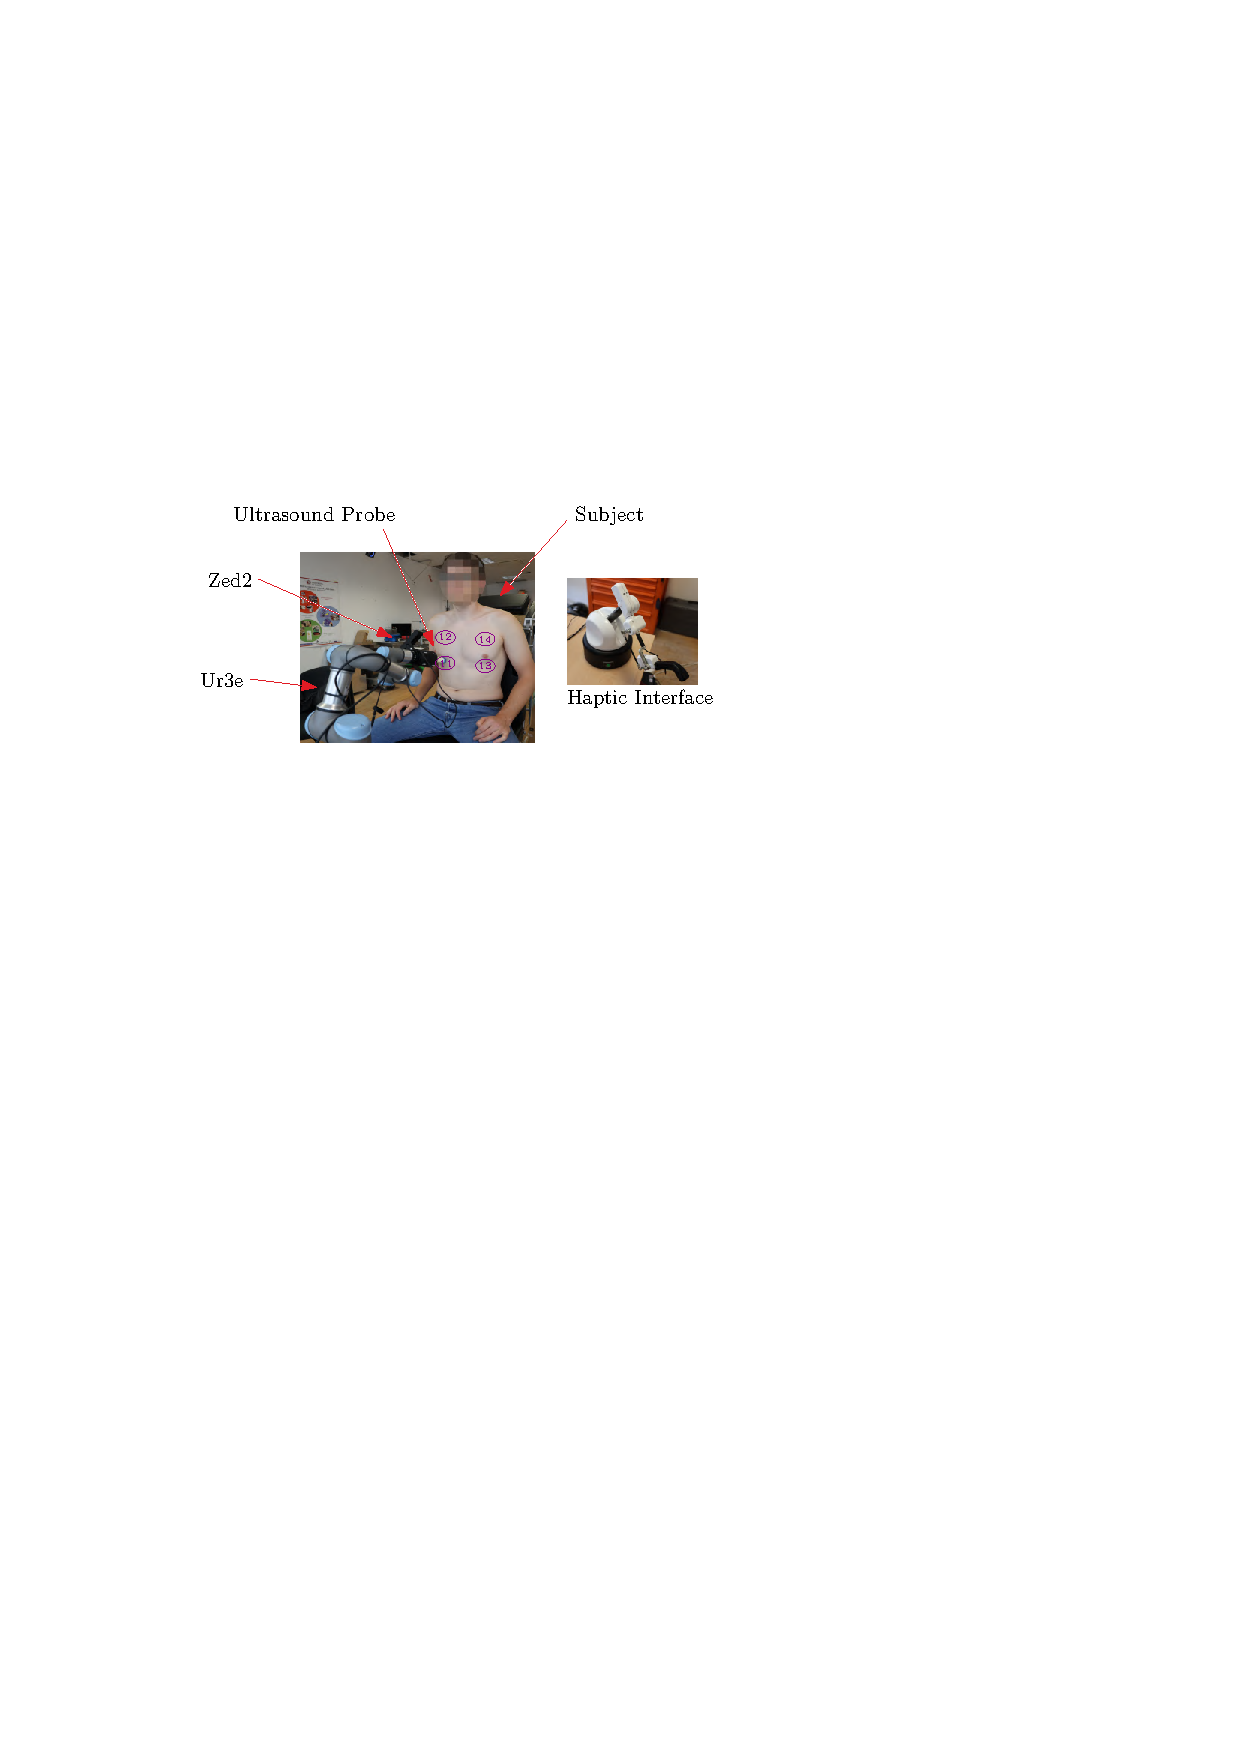
\includegraphics[width=1\linewidth]{images/experiments/setup.pdf}
%     \caption{Experimental setup: a volunteer male healthy patient sit on an hospital bed and is examinated by a robot arm controlled by the practioner through an haptic interface. The frontal scanning areas of the lung ultrasound protocol considered are marked in purple.   }
%     \label{fig:experiments:setup}
% \end{figure}
Before performing the 4-points frontal examination in accordance with the methodology delineated by Soldati et al.~\cite{Soldati2020ProposalCOVID-19} (see ~\autoref{fig:experiments:setup}), we performed a study with only 2 points: 11 and 12, similarly to the second experiment.
%the acquisition is conducted at the four frontal points, namely 11, 12, 13 and 14, shown .% 
The acquisition was deemed valid at each point if the pleural line was
visible for a minimum of $90\%$ of its horizontal extension in the
image (see~\autoref{fig:experiments:pleural} for a visual reference).  Before the
experiment starts, the operator tested for $10$ minutes the system to
become acquainted with it and to avoid the introduction of any bias
into the initial measurements. Furthermore, the tests with and without
VF were alternated, to prevent major influence due to
the indirect training of the task from the
subject with a total of $10$ attempts (5 with VF and 5
without). The mean and standard deviation (in seconds) of the error
between the examination with and without the VF for the
2-points study with operator \#1 are reported in the first row of
\autoref{tab:experiments:scan_times}.
\begin{table}
    \centering
    \caption{Mean examination duration [$s$] with and without the proposed shared control framework}
    \begin{tabular}{ccc}
    \toprule
       \sc{Experiment} & \sc{w/ VF, Mean} $\pm$ \sc{std} &        \sc{w/o VF, Mean} $\pm$ \sc{std} \\
       \midrule
       2-pts, operator \#1 & $35 \pm 8$ & $50 \pm 13$\\
       4-pts, operator \#2 & $100 \pm 15$ & $135 \pm 9$ \\
       \bottomrule
    \end{tabular}
    \label{tab:experiments:scan_times}
    \vspace{4mm}
\end{table}

Data shows a marked reduction of 30\% in the total execution time of the examination when the VF were used and lower standard deviation, indicating higher repeatability. We then extended this experiments by performing the 4-points examination (areas 11-12-14-13) with the same modalities. To further reduce the bias, we also change the operator. The 4-points protocol mean and standard deviation duration times with and without our assistance method for operator \#2 are reported in the second row of \autoref{tab:experiments:scan_times}. As we can observe, the total time was reduced by approximately 26\%, comparable to the 2-points attempts with a different operator. Overall, the 2-points and 4-points evaluations remark a promising improvement in the total execution time. 
\noindent
Furthermore, the operators reported a reduced cognitive effort and an
increased confidence during free motion, attributed to the easier
identification of target points. Another limitation identified by the
user when relying solely on the RGB image for feedback is the
occlusion of the camera view by the end effector in certain
configurations, which complicates the interaction process. This issue,
however, was not critical when VF were employed, since,
thanks to the 3D visual feedback, the position of the probe in the
ribs region remained consistently visible.



\begin{figure}[t!]
    \centering
    \hspace{21mm}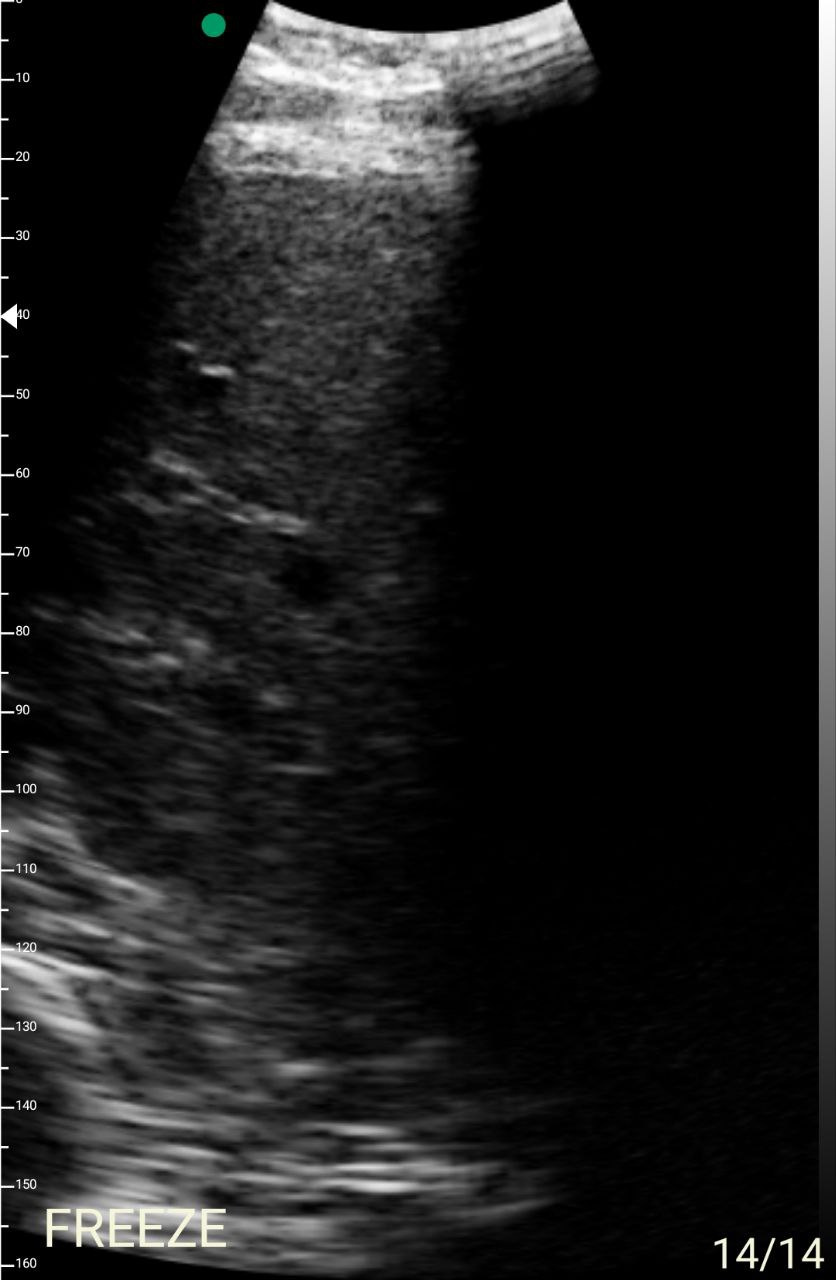
\includegraphics[trim=0cm 0cm 0cm 0cm,clip,height=7cm]{images/experiments/pleural_bad.jpg}
    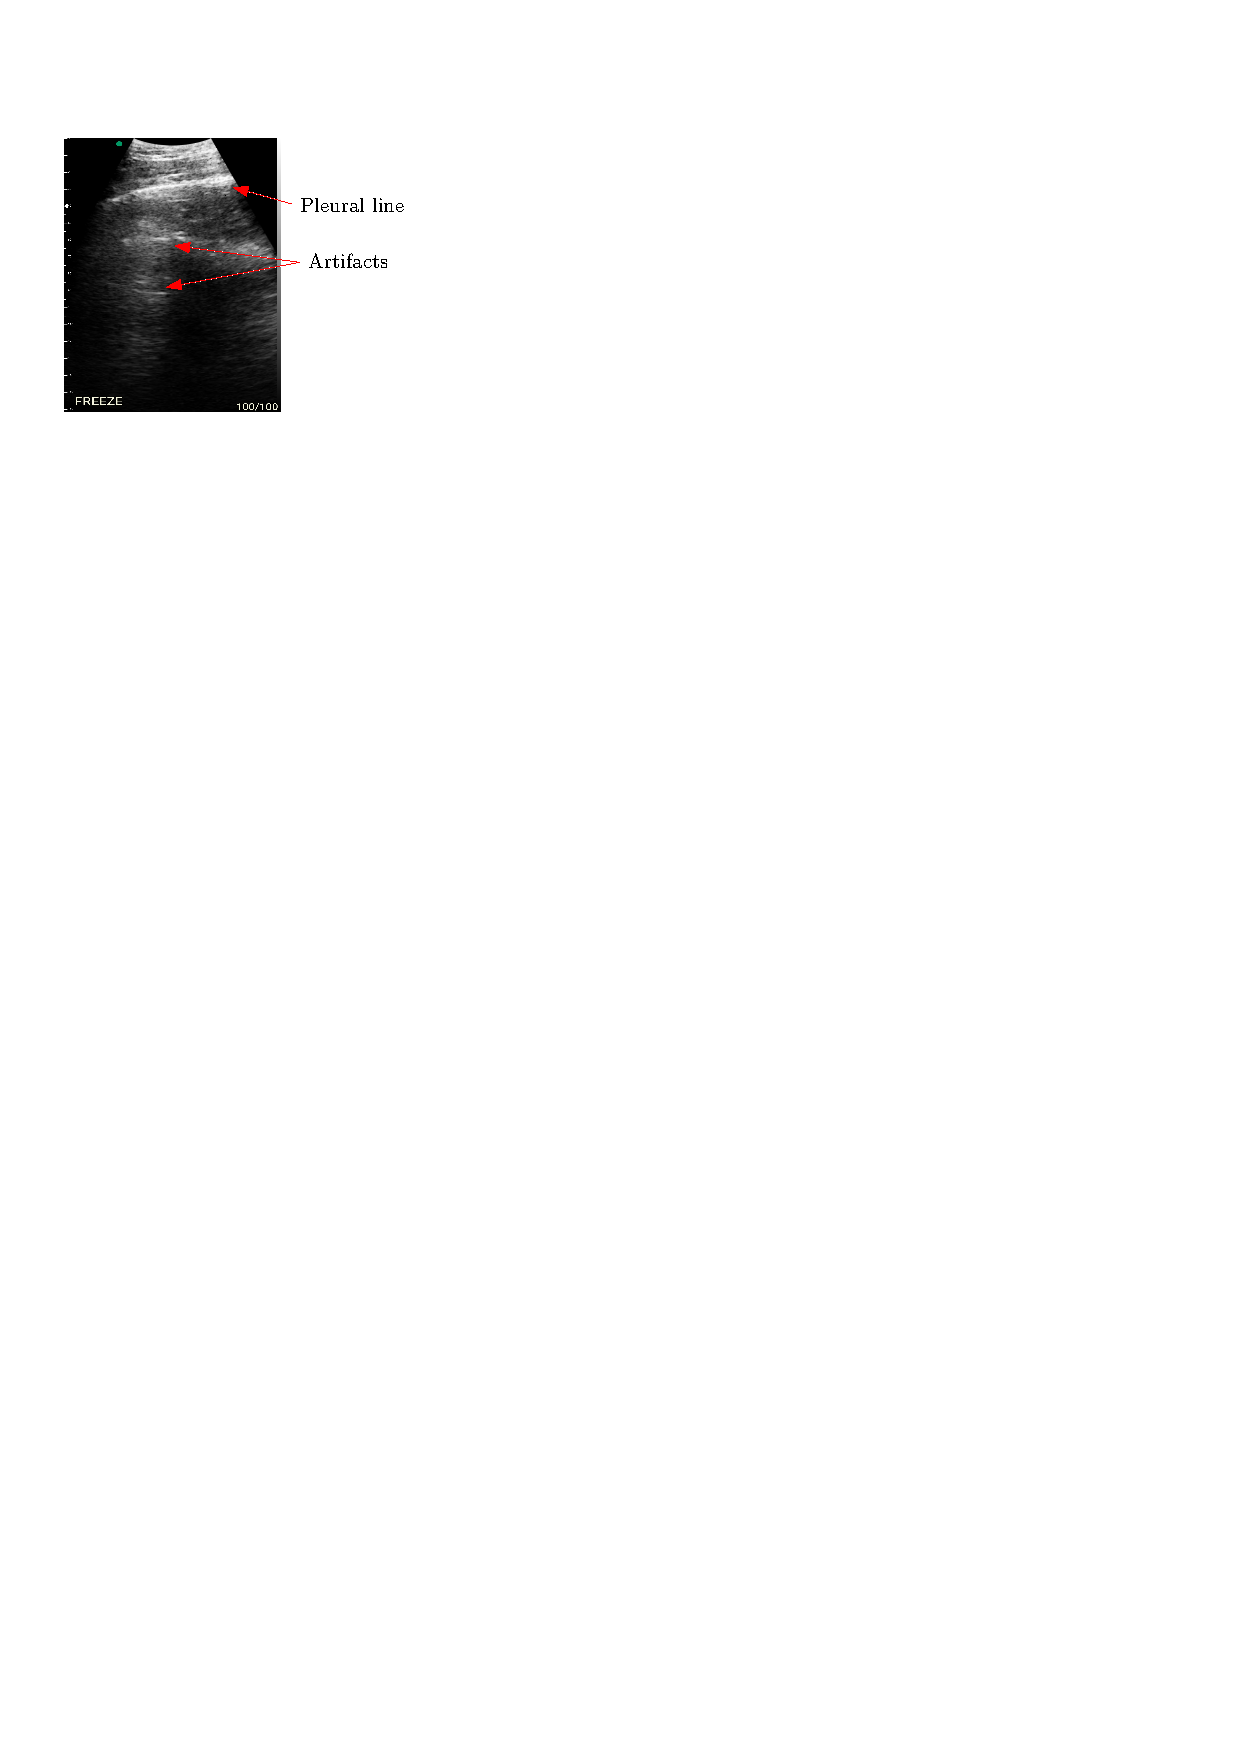
\includegraphics[trim=0cm 0cm 0cm 0cm,clip,height=7cm,width=7.5cm]{images/experiments/pleural.pdf}
    \caption{Examples of lung ultrasound images sampled from the probe attached at the end effector of the robot: (left) rib shadow, (right) full pleural line}
    \label{fig:experiments:pleural}
\end{figure}

% \clearpage
% \newpage
% \mbox{}
% \clearpage
